\documentclass{vhdl-assignment}

\title{Assignment 4}
\date{October 9, 2023}

\begin{document}
\maketitle
\thispagestyle{fancy}

Design code, testbench and simulation the following module

\begin{problem}{4-bit Ripple Carry Counter}
    \note{Using T - flipflop (Structural model) that you designed in Assignment 3.}

    \begin{figure}[H]
        \centering
        \begin{circuitikz}
            \node[T_FF_neg] (T0) at (0,0) {T0};
            \node[T_FF_neg] (T1) at (3,0) {T1}; 
            \node[T_FF_neg] (T2) at (6,0) {T2};
            \node[T_FF_neg] (T3) at (9,0) {T3};

            \node (CLK) at ($(T0.pin 2) + (-1,0)$) {CLK};
            \node (RST) at ($(CLK) + (0,-3)$) {RST};

            \node (Q0) at ($(T0.pin 6)+(0,2)$) {Q0};
            \node (Q1) at ($(T1.pin 6)+(0,2)$) {Q1};
            \node (Q2) at ($(T2.pin 6)+(0,2)$) {Q2};
            \node (Q3) at ($(T3.pin 6)+(0,2)$) {Q3};

            \draw (CLK) -- (T0.pin 2);
            \draw (T0.pin 6) |- (T1.pin 2);
            \draw (T1.pin 6) |- (T2.pin 2);
            \draw (T2.pin 6) |- (T3.pin 2);

            \draw (RST) -- ($(RST)!(T0.down)!($(RST)+(1,0)$)$) |- (T0.down);
            \draw (RST) -- ($(RST)!(T1.down)!($(RST)+(1,0)$)$) |- (T1.down);
            \draw (RST) -- ($(RST)!(T2.down)!($(RST)+(1,0)$)$) |- (T2.down);
            \draw (RST) -- ($(RST)!(T3.down)!($(RST)+(1,0)$)$) |- (T3.down);

            \draw (Q0) -- (T0.pin 6);
            \draw (Q1) -- (T1.pin 6);
            \draw (Q2) -- (T2.pin 6);
            \draw (Q3) -- (T3.pin 6);
        \end{circuitikz}
        \caption{4-bit Ripple Carry Counter}
    \end{figure}
\end{problem}

\begin{problem}{4-bit Gray Counter}
    \note{The counter has synchrounous reset}
\end{problem}

\begin{problem}{BCD to 7 Segment Display Decoder}
    \begin{figure}[H]
        \centering
        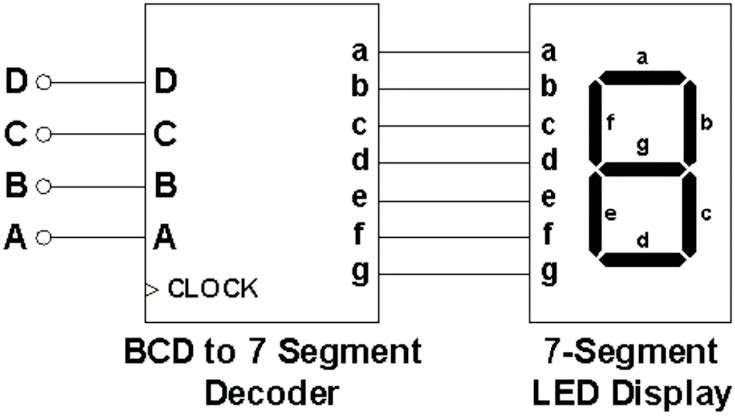
\includegraphics{assets/GrayCounter.jpg}
    \end{figure}
\end{problem}

\end{document}